\chapter{Теоретические исследования}
\label{chapter2}

В данной главе будут представлены основные результаты работы. Сначала будет рассмотрен основные кандидаты для
гибридизации. Затем будет представлен анализ работы кандидатов на разных входных данных. Потом будет сделано
некоторое предположение на основании экспериментов и на его основе сформулирован алгоритм гибридизации.

\section{Анализ существующих алгоритмов}

В качестве основного кандидата для гибридизации был выбран алгоритм ``разделяй и властвуй''. Причин для этого две:

\begin{enumerate}
 \item Данный алгоритм работает лучше большинства алгоритмов. Благодаря этому гибридный алгоритм тоже будет работать эффективно.
 \item Данный алгоритм рекурсивно запускает себя в процессе своей работы. Это порождает точки возможного подключения других алгоритмов.
\end{enumerate}

Вторым кандидатом стал алгоритм Роя по следующим причинам:

\begin{enumerate}
 \item Судя по разобранным авторами этого алгоритма случаям, данный алгоритм в лучших случаях может работать крайне эффективно, лучше других известных алгоритмов.
 \item Нет строгого доказательства времени работы данного алгоритма, только результаты экспериментальных запусков. Данная работа является отличной возможностью сравнить этот алгоритм с другими существующими.
\end{enumerate}

Далее в данной работе для краткости алгоритм Буздалова будет называться ``Fast'', потому что он считается алгоритмом
быстрой недоминирующей сортировки, а алгоритм Роя -- ``BOS'', так как его автор называет свой алгоритм лучшим
алгоритмом недоменирующей сортировки (Best Order Sort).

Был проведен ряд экспериментов, сравнивающий времена работы данных алгоритмов. В данных экспериментах сравнивалось
среднее время работы каждого алгоритма на данных, имеющих разные размера и размерности. Для визуального представления
и анализа были нарисованы графики функции $\frac{T_{BOS} - T_{Fast}}{T_{MAX}}$, где $T_{BOS}$ -- время работы алгоритма
BOS, $T_{Fast}$ -- время работы алгоритма Fast, а $T_{MAX} = \max(T_{BOS}, T_{Fast})$. Чем меньше значение этой
функции, тем эффективнее работает алгоритм BOS. Если функция принимает значение ноль, то оба алгоритма работают
одинаково эффективно.

Эксперименты проводились для разных $N$ и $M$ -- числа и размерности точек соответственно. Также использовались
разные способы генерации входных данных:

\begin{enumerate}
 \item Случайные точки в гиперкубе.
 \item Случайно сгенерированные точки, имеющие фиксированное число фронтов.
\end{enumerate}

Для подсчета времени работы алгоритма на каждых данных проводилось несколько его запусков. Время засекалось с помощью
Java-библиоетки %TODO: назвать библиотеку
Если суммарное время даже нескольких запусков было очень маленьким и имело малую точность, алгоритм запускался на
этих значениях еще больше раз, пока не достигалась желаемая точность измерений.

Ниже на рисунке~\ref{experiment} приведены результаты зависимости относительной разницы во времени работы алгоритмов
от размера водных данных для разных размерностей и способов генерации входных данных.


\begin{figure}
\begin{center}
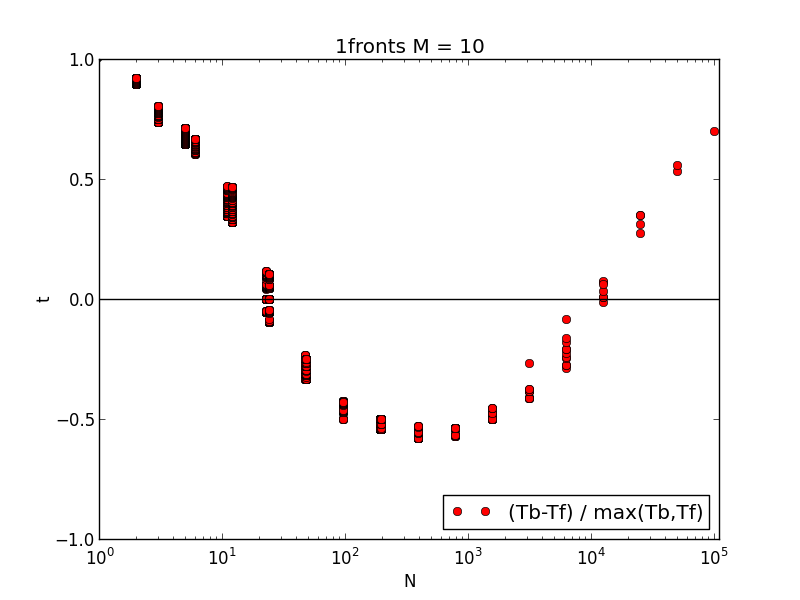
\includegraphics[width=8cm]{pic/bos_fast.png}
\caption{Относительная разность времени работы кандидатов для гибридизации на одном из видов входных данных}
%при разных способах генерации входных
%данных: $CUBE$ -- случайные точки в гиперкубе, $FN$ -- случайные точки, имеющие $N$ фронтов}
\label{experiment}
\end{center} % TODO
\end{figure}

Результаты экспериментов получились очень сильно зашумленными, поэтому для того, чтобы лучше увидеть зависимость
времени работы алгоритмов от размера входных данных, был применен метод интерквартериальных интервалов. Он
заключается в том, что в каждом небольшом промежутке аргумента (в нашем случае это число точек сортируемого
множества $N$) удаляется половина точек, которые находятся ближе к крайним значениям. Применение данного метода
дало увидеть более четкую картину происходящего.

Из данных, полученных в результате экспериментов, можно сделать некоторые выводы. Самым главным утвержеднием
является то, что алгоритм Fast работает быстрее, чем BOS при очень малых и очень больших размерах входных данных.
Однако сучществует некоторый интервал значений $N$, при котором алгоритм BOS работает значительно лучше. Причем
можно рассмотреть зависимость левой и правой границ в зависимости от размерности задачи и способа генерации даных.
Графики этих зависимостей представлены на расунке~\ref{borders}.

\begin{figure}
\begin{center}
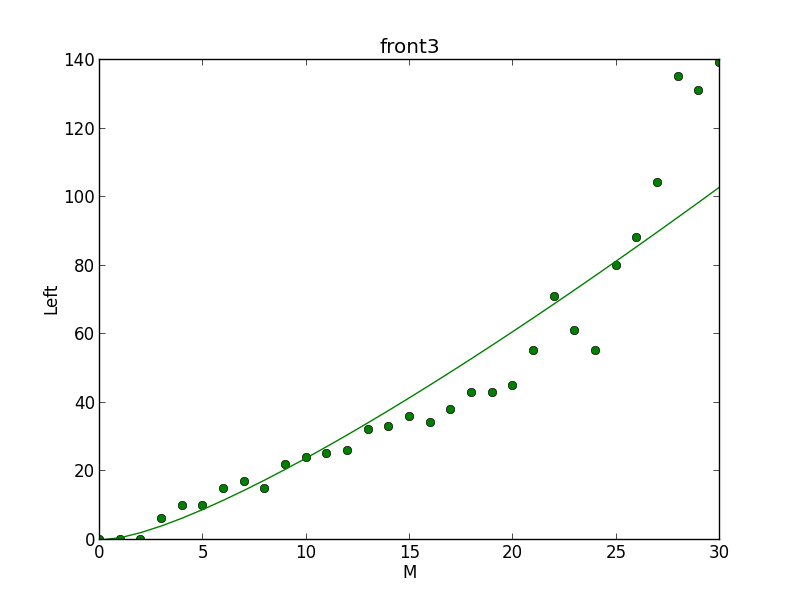
\includegraphics[width=8cm]{pic/left.png}
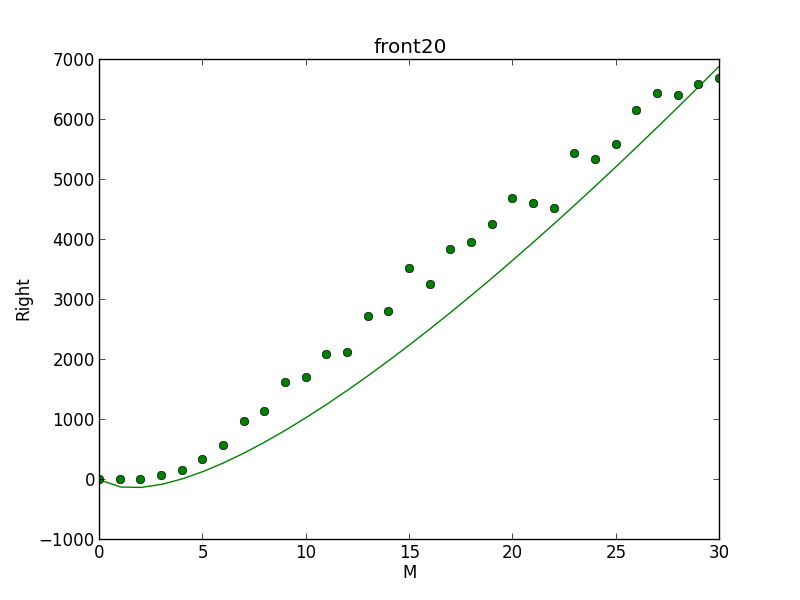
\includegraphics[width=8cm]{pic/right.png}
\caption{Зависимость левой и правой границы эффективности BOS от размерности задачи}
%:$CUBE$ -- случайные точки в гиперкубе, $FN$ -- случайные точки, имеющие $N$ фронтов}
\label{borders}%TODO
\end{center}
\end{figure}

Нижняя и верхняя границы почти всегда зависят только от размерности и слабо зависят от числа фронтов. Зависимость
от числа фронтов проявляется только у верхней границы: на графике для случайных точек в гиперкубе виден большой
скачок при небольших размерностях. Это объясняется тем, что с ростом размерности при одинаковом числе входных
точек значительно падает число фронтов, но при малых размерностях оно может быть большим. Таким образом, было
выдвинуто предположение, что нижняя граница зависит от размерности $M$ по закону $l(d) = c_1 \cdot d \cdot \ln(d + 1)$,
а верхняя -- $r(d) = c_2 \cdot d \cdot (\ln^{0.9}(d + 1) - 1.5)$, где $c_1$  и $c_2$ -- константы, зависящие от
машины, на которой работает алгоритм, а также от ее загруженнсоти. В случае машины, на которой запускались
эксперименты, $c_1 \approx 1$, а $c_2 \approx 150$.

\section{Предлагаемая схема гибридизации}

Как уже говорилось выше, мы можем воспользоваться тем, что алгоритм Fast может во время рекурсивного запуска
себя запускать другой алгоритм недоминирующей сортировки, в нашем случае BOS. Однако он должен уметь быстро
определять, какой алгоритм в данном случае лучше запустить. Если решение будет занимать много времени, то
алгоритм будет работать дольше, чем лучший из гибридиируемых алгоритмов.

Один из способов быстро выбрать алгоритм -- основываясь на размерах и размерности данных и на результатах
экспериментов сказать, какой алгоритм на этих данных отработает быстрее, и выбрать его. Вероятно, это не самый
эффективный способ выбора момента переключения. Может случиться, что если алгоритм Fast сделает еще несколько шагов
вглубь, создав множества поменьше, то алгоритм BOS на них отработает значительно лучше, и время всего алгоритма в
целом будет значительно меньше. Однако момент оптимального переключения неизвестен, а также очень трудно находим
с помощью экспериментов из больших шумов во времени работа гибрида.

Таким образом, прелагается следующий гибридный алгоритм:
\begin{enumerate}
 \item Запускаем алгоритм Fast.
 \item Перед каждым запуском $NDHelperA$ проверяем, не лучше ли на данном размере данных и размерности работает $BOS$.
 \item Запускаем лучший из двух алгоритм.
\end{enumerate}

\subsection{Проблемы}

В описанном алгоритме существуют две основные проблемы, которые сформулированы в данном подразделе.

\subsubsection{Момент переключения}

Первой проблемой является то, что заранее не может быть известно, какой алгоритм лучше на конкретных данных. Не
может быть дано даже теоретических оценок зависимости лучшего алгоритма от размера и размерности входных данных,
так как они отсутствуют для алгоритма BOS. Однако благодаря тому, что по результатам экспериментов, для каждой
размерности входных точек, алгоритм BOS работает лучше только на определенном интервале значений числа входных
точек, момент переключения легко вычислять по тому, находится ли текущий размер сортируемого множества в данном
интервале.

При этом до сих пор остается проблемой вычиление границ интервала, на котором эффективнее работает BOS. Решение
данной проблемы описано в следующем подразделе.

\subsubsection{Предпоставленные ранги}

Второй проблемой является то, что алгоритм Fast перед рекурсивным запуском себя расставляет минимальные ранги для
точек множества, на котором собирается запускаться. Алгоритм BOS не предусматривает возможности наличия у точек
минимально возможных рангов, поэтому требуется модификация этого алгоритма.

\subsection{Выбор момента переключения}

Как уже было сказано, основная проблема выбора момента переключения заключается в нахождении границ интервала, на
котором BOS работает лучше, чем алгоритм Fast. Эти границы имеют завсимость от размерности входных данных, а также
от можности машины, на которой запускается алгоритм. Ниже описаны методы нахождения этих зависимостией.

\subsubsection{Зависимость от данных}

В результате экспериментов было выявлено, что левая и правая граница интервала размеров входных данных, на
котором BOS  работает эффективнее, чем Fast, зависит от размерности входных точек, а также иногда от числа различных
рангов во входном множестве.

Левая граница интервала почти не зависит от числа рангов, а ее поведение завимиости от размерности задачи достаточно
хорошо описывается формулой $1/5 M \ln (M + 1)$.

С правой границей все гораздо хуже: она ведет себя непредсказуемо даже для фиксированного числа рангов во входных
данных. Для решения данной проблемы требуется научиться считать эту границу перед запусками алгоритма.

\subsubsection{Выбор времени переключения}

Было предложено решение проблемы зависимости границ от данных: перед запуском алгоритма сначала искать границы
эффективного интервала алгоритма BOS на случайных данных. Для этого на размерностях не более $M$, где $M$ -- это
максимально возможная размерность, которая понадобится в задаче, запускается процедура нахождения границ. Она состоит
из трех этапов: поиск размера данных, на котором алгоритм BOS максимально эффективнее алгоритма Fast, затем поиск
левой границы и, наконец, поиск правой границы.

Первый этап реализован с помощью троичного поиска. Как мы видим из результатов экспериментов, производная функции
относительной разницы времени работы алгоритмов имеет всего лишь один ноль производной. Таким образом, применив
троичный поиск на интервале $[0; 2 \cdot 10^4]$, мы сможем найти минимум этой функции. Правая граница интервала поиска
выбрана так, чтобы по результатам экспериментов она всегда значительно превышала правую границу интервала
эффективности BOS, что гарантирует нам успешное нахождение минимума.

Стоит заметить, что так как модуль производной функции сильно падает с ростом $N$. Также мы можем в достаточной мере
пренебречь точностью занчения границ при достаточно больших значениях входных данных. Из этого можно сделать вывод,
что троичный поиск можно производить по логарифмической шкале, а не по линейной. То есть в качестве точек, в которых
считается относительная разница времени работ алгоритмов, лучше брать не $\frac{2l + r}{2}$ и $\frac{l + 2r}{2}$, где
$l$ и $r$ -- текущие границы интервала поиска, а $e^{\frac{2\ln l + \ln r}{2}}$ и $e^{\ln\frac{\ln l + 2 \ln r}{2}}$.

Для вычисления функции относительной разницы времени работы алгоритмов троичный поиск считает ее сезнее значение по 15
запускам алгоритмов на разных случайно сгенерированных данных.

Это порождает некоторые шумы значений функции, поэтому троичный поиск не всегда может быть уверенным, что если значения
функции в двух средних точках равны, то ему надо идти в средний интервал. Для того, чтобы определить, в какую сторону
ему следует идти, он сравнивает разницу значений в средних точках и на границах, и идет туда, где эта разница меньше.

После нахождения размера входных данных $X$, на котором алгоритм BOS имеет максимальную относительную эффективность,
процедура поиска границ приступает к поиску границ иинтервала эффективности BOS с помощью двоичного поиска на
интервалах $[1;X]$ и $[X;2\cdot10^4]$, для левой и правой границ соответственно.

Функция относительной разницы времени работы алгоритмов считается так же, как и в троичном поиске. Из-за этого
появляются шумы, поэтому мы удовлетворяемся значением границы, на котором относительная разница работы абсолютно
не превосходит $\eps = 0.01$.

Описанная процедура способна достаточно быстро находить границы интервала размеров входных данных, на котором стоит
запускать BOS, что необходимо для работы гибридного алгоритма.

%TODO Описать подгонку функций для границ под данные.

\subsubsection{Зависимость от оборудования}

Также было замечено, что значения границ могут варьироваться от одной вычислительной машины к другой. Даже на одной
машине в зависимости от ее загруженности в текущий момент эти границы могут немного сдвигаться. Это вызывает
некоторые сложности из-за неактуальности уже подсчитанных границ.

\subsubsection{Построение стратегии переключения на ходу}

Предлагается в начале каждого запуска программы, которая использует алгоритм недоминирующей сортировки, производить
подгонку границ. Это займет некоторое время, однако если программа будет использовать донастроенный алгоритм
достаточно много раз, то итоговый выигрыш по времени может быть значительным. Если вспомнить, что недоминирующая
сортировка используется в основном в алгоритмах многокритериальной оптимизации, то можно сказать, что эта ситуация
возникает достаточно часто.

Также для каждого значения размерности существуют заранее посчитанные интервалы возможных значений границ, что
ускоряет поиск их точных значений.

\subsection{Модификация алгоримтма Роя}
Алгоритм Буздалова и др перед рекурсивным запуском себя расставляет минимальные ранги для
точек множества, на котором собирается запускаться. Алгоритм BOS не предусматривает возможности наличия у точек
минимально возможных рангов, поэтому требуется модификация этого алгоритма.
В момент определения ранга алгоритм BOS перебирает возможные ранги и определяет минимальный возможный. Для того, чтобы
учесть заранее проставленный ранг, надо начинать перебор с уже проставленного ранга, а не с 0.

%TODO

